% Options for packages loaded elsewhere
\PassOptionsToPackage{unicode}{hyperref}
\PassOptionsToPackage{hyphens}{url}
\PassOptionsToPackage{dvipsnames,svgnames,x11names}{xcolor}
%
\documentclass[
  letterpaper,
  DIV=11,
  numbers=noendperiod]{scrartcl}

\usepackage{amsmath,amssymb}
\usepackage{iftex}
\ifPDFTeX
  \usepackage[T1]{fontenc}
  \usepackage[utf8]{inputenc}
  \usepackage{textcomp} % provide euro and other symbols
\else % if luatex or xetex
  \usepackage{unicode-math}
  \defaultfontfeatures{Scale=MatchLowercase}
  \defaultfontfeatures[\rmfamily]{Ligatures=TeX,Scale=1}
\fi
\usepackage{lmodern}
\ifPDFTeX\else  
    % xetex/luatex font selection
  \setmainfont[]{Inter}
  \setsansfont[]{Inter}
\fi
% Use upquote if available, for straight quotes in verbatim environments
\IfFileExists{upquote.sty}{\usepackage{upquote}}{}
\IfFileExists{microtype.sty}{% use microtype if available
  \usepackage[]{microtype}
  \UseMicrotypeSet[protrusion]{basicmath} % disable protrusion for tt fonts
}{}
\makeatletter
\@ifundefined{KOMAClassName}{% if non-KOMA class
  \IfFileExists{parskip.sty}{%
    \usepackage{parskip}
  }{% else
    \setlength{\parindent}{0pt}
    \setlength{\parskip}{6pt plus 2pt minus 1pt}}
}{% if KOMA class
  \KOMAoptions{parskip=half}}
\makeatother
\usepackage{xcolor}
\setlength{\emergencystretch}{3em} % prevent overfull lines
\setcounter{secnumdepth}{5}
% Make \paragraph and \subparagraph free-standing
\ifx\paragraph\undefined\else
  \let\oldparagraph\paragraph
  \renewcommand{\paragraph}[1]{\oldparagraph{#1}\mbox{}}
\fi
\ifx\subparagraph\undefined\else
  \let\oldsubparagraph\subparagraph
  \renewcommand{\subparagraph}[1]{\oldsubparagraph{#1}\mbox{}}
\fi


\providecommand{\tightlist}{%
  \setlength{\itemsep}{0pt}\setlength{\parskip}{0pt}}\usepackage{longtable,booktabs,array}
\usepackage{calc} % for calculating minipage widths
% Correct order of tables after \paragraph or \subparagraph
\usepackage{etoolbox}
\makeatletter
\patchcmd\longtable{\par}{\if@noskipsec\mbox{}\fi\par}{}{}
\makeatother
% Allow footnotes in longtable head/foot
\IfFileExists{footnotehyper.sty}{\usepackage{footnotehyper}}{\usepackage{footnote}}
\makesavenoteenv{longtable}
\usepackage{graphicx}
\makeatletter
\def\maxwidth{\ifdim\Gin@nat@width>\linewidth\linewidth\else\Gin@nat@width\fi}
\def\maxheight{\ifdim\Gin@nat@height>\textheight\textheight\else\Gin@nat@height\fi}
\makeatother
% Scale images if necessary, so that they will not overflow the page
% margins by default, and it is still possible to overwrite the defaults
% using explicit options in \includegraphics[width, height, ...]{}
\setkeys{Gin}{width=\maxwidth,height=\maxheight,keepaspectratio}
% Set default figure placement to htbp
\makeatletter
\def\fps@figure{htbp}
\makeatother

\usepackage{amsmath, xparse}
\usepackage{fancyvrb, fvextra}
\usepackage{bm}
\usepackage{svg}
\usepackage{listings}
\usepackage{xifthen}
\DefineVerbatimEnvironment{Highlighting}{Verbatim}{breaklines,commandchars=\\\{\}}
\lstset{basicstyle=\ttfamily\footnotesize,breaklines=true}
\KOMAoption{captions}{tableheading}
\makeatletter
\makeatother
\makeatletter
\makeatother
\makeatletter
\@ifpackageloaded{caption}{}{\usepackage{caption}}
\AtBeginDocument{%
\ifdefined\contentsname
  \renewcommand*\contentsname{Table of contents}
\else
  \newcommand\contentsname{Table of contents}
\fi
\ifdefined\listfigurename
  \renewcommand*\listfigurename{List of Figures}
\else
  \newcommand\listfigurename{List of Figures}
\fi
\ifdefined\listtablename
  \renewcommand*\listtablename{List of Tables}
\else
  \newcommand\listtablename{List of Tables}
\fi
\ifdefined\figurename
  \renewcommand*\figurename{Figure}
\else
  \newcommand\figurename{Figure}
\fi
\ifdefined\tablename
  \renewcommand*\tablename{Table}
\else
  \newcommand\tablename{Table}
\fi
}
\@ifpackageloaded{float}{}{\usepackage{float}}
\floatstyle{ruled}
\@ifundefined{c@chapter}{\newfloat{codelisting}{h}{lop}}{\newfloat{codelisting}{h}{lop}[chapter]}
\floatname{codelisting}{Listing}
\newcommand*\listoflistings{\listof{codelisting}{List of Listings}}
\makeatother
\makeatletter
\@ifpackageloaded{caption}{}{\usepackage{caption}}
\@ifpackageloaded{subcaption}{}{\usepackage{subcaption}}
\makeatother
\makeatletter
\@ifpackageloaded{tcolorbox}{}{\usepackage[skins,breakable]{tcolorbox}}
\makeatother
\makeatletter
\@ifundefined{shadecolor}{\definecolor{shadecolor}{rgb}{.97, .97, .97}}
\makeatother
\makeatletter
\makeatother
\makeatletter
\makeatother
\ifLuaTeX
  \usepackage{selnolig}  % disable illegal ligatures
\fi
\IfFileExists{bookmark.sty}{\usepackage{bookmark}}{\usepackage{hyperref}}
\IfFileExists{xurl.sty}{\usepackage{xurl}}{} % add URL line breaks if available
\urlstyle{same} % disable monospaced font for URLs
\hypersetup{
  colorlinks=true,
  linkcolor={blue},
  filecolor={Maroon},
  citecolor={Blue},
  urlcolor={Blue},
  pdfcreator={LaTeX via pandoc}}

\author{}
\date{}

\begin{document}
\begin{titlepage}

    \newcommand{\HRule}{\rule{\linewidth}{0.5mm}}
    
    \center
    
    \vspace{10cm}

    \textsc{\LARGE Gwinnett School of Math, Science, and Technology }\\[0.3cm]
    
    \vspace{0.5cm}

    \HRule \\[0.4cm]
    { \huge \bfseries AP Physics: Mechanics/Electricity \& Magnetism Notes}\\[0.03cm]
    \HRule \\[1.5cm]
    
    \begin{minipage}{0.4\textwidth}
    \begin{flushleft} \Large
    Anish Goyal \\3rd/4th Period
    \end{flushleft}
    \end{minipage}
    ~
    \begin{minipage}{0.4\textwidth}
    \begin{flushright} \Large
    Jeffrey Burmester\\Educator
    \end{flushright}
    \end{minipage}\\[1cm]
    
    {\huge 2023-2024}\\[1cm]
    
    
\includegraphics{img/logo.png}\\
    \vfill
    \end{titlepage}
\newpage

\ifdefined\Shaded\renewenvironment{Shaded}{\begin{tcolorbox}[boxrule=0pt, enhanced, interior hidden, borderline west={3pt}{0pt}{shadecolor}, breakable, sharp corners, frame hidden]}{\end{tcolorbox}}\fi

\renewcommand*\contentsname{Table of Contents}
{
\hypersetup{linkcolor=}
\setcounter{tocdepth}{4}
\tableofcontents
}
\newpage{}

\hypertarget{kinematics}{%
\section{Kinematics}\label{kinematics}}

\hypertarget{variables}{%
\subsection{Variables}\label{variables}}

\textbf{Position}

\begin{itemize}
\tightlist
\item
  Typically given by the variable \(x\)
\end{itemize}

\textbf{Time}

\begin{itemize}
\tightlist
\item
  Typically given by the variables \(t\)
\end{itemize}

\textbf{Displacement}

\begin{itemize}
\tightlist
\item
  Defined as the change in position (\(X_f - X_i\))
\item
  Given by the variable \(\Delta x\)
\end{itemize}

\textbf{Distance}

\begin{itemize}
\tightlist
\item
  You have to take the magnitude of vectors for every time you change
  position
\item
  \(S = |x_2 - x_1| + |x_1 - x_0| + ...\)
\end{itemize}

\textbf{Average Velocity}

\begin{itemize}
\tightlist
\item
  Defined as the change in displacement over time
\item
  \(\frac{\Delta x}{\Delta t} = V_\text{avg} = \bar{V}\)
\end{itemize}

\textbf{Velocity}

\begin{itemize}
\tightlist
\item
  Defined as the change in displacement as time approaches 0
\item
  \(\lim_{\Delta t \to 0} \frac{\Delta x}{\Delta t} = \frac{dx}{dt} = V\)
\end{itemize}

\textbf{Average Acceleration}

\begin{itemize}
\tightlist
\item
  Defined as the change in velocity over time
\item
  \(\frac{\Delta V}{\Delta t} = A_\text{avg} = \bar{A}\)
\end{itemize}

\textbf{Acceleration}

\begin{itemize}
\tightlist
\item
  Defined as the change in velocity as time approaches 0
\item
  \(a = \lim_{\Delta t \to 0} \frac{\Delta V}{\Delta t} = \frac{dV}{dt} = \frac{d^2x}{dt^2}\)
\end{itemize}

\textbf{Speed} - \(\text{Speed} = \frac{S}{t}\) - Alternatively, when
referring to vectors: \(\text{Speed} = ||\vec{V}||\)

\hypertarget{kinematics-velocity-and-position-definitions-0803-homework}{%
\subsection{Kinematics: Velocity and Position Definitions (08/03
Homework)}\label{kinematics-velocity-and-position-definitions-0803-homework}}

The position versus time for a certain particle moving along the x axis
is shown in the figure below. Find the average velocity in the following
time intervals.

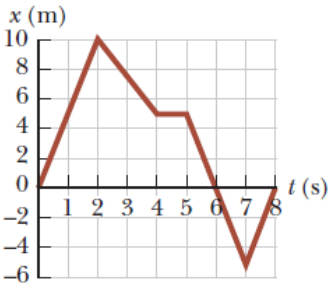
\includegraphics{img/Kinematics Velocity and Position HW/problem1.png}

\begin{enumerate}
\def\labelenumi{(\alph{enumi})}
\tightlist
\item
  0 to 2s
\end{enumerate}

\begin{itemize}
\tightlist
\item
  5.000m/s
\end{itemize}

\begin{enumerate}
\def\labelenumi{(\alph{enumi})}
\setcounter{enumi}{1}
\tightlist
\item
  0 to 4s
\end{enumerate}

\begin{itemize}
\tightlist
\item
  1.250m/s
\end{itemize}

\begin{enumerate}
\def\labelenumi{(\alph{enumi})}
\setcounter{enumi}{2}
\tightlist
\item
  2 to 6s
\end{enumerate}

\begin{itemize}
\tightlist
\item
  -2.500m/s
\end{itemize}

\begin{enumerate}
\def\labelenumi{(\alph{enumi})}
\setcounter{enumi}{3}
\tightlist
\item
  1 to 7s
\end{enumerate}

\begin{itemize}
\tightlist
\item
  -1.667m/s
\end{itemize}

\begin{enumerate}
\def\labelenumi{(\alph{enumi})}
\setcounter{enumi}{4}
\tightlist
\item
  0 to 7s
\end{enumerate}

\begin{itemize}
\tightlist
\item
  -0.714s
\end{itemize}

\hypertarget{derivative-relationships}{%
\subsection{Derivative Relationships}\label{derivative-relationships}}

\textbf{Acceleration and Velocity}

\begin{itemize}
\tightlist
\item
  \(a = \frac{dV}{dt}\)
\item
  \(V = \frac{dx}{dt}\)
\item
  \(\int{V_0}{V} dV = \int_{0}^{t} a dt\)
\item
  \(V\rvert_{V_0}^{V} = a\rvert_{0}^{t}\)
\item
  \(V - V_0 = at\)
\item
  \(V = at + V_0\)
\end{itemize}

\textbf{Acceleration and Position}

\begin{itemize}
\tightlist
\item
  \(V = \frac{dx}{dt}\)
\item
  \(\int_{0}^{x} V dt = \int_{0}^{t} at + V_0 dt\)
\item
  \(x\rvert_{0}^{x} = \frac{1}{2}at^2 + V_0t\rvert_{0}^{t}\)
\item
  \(x = \frac{1}{2}at^2 + V_0t\)
\end{itemize}

\emph{If initial time or position is not zero:}

\begin{itemize}
\tightlist
\item
  \(x-x_0 = V_0(t-t_0) + \frac{1}{2}a(t-t_0)^2\)
\end{itemize}

\hypertarget{given-x4t4---6t-find-a-when-t2.}{%
\subsubsection{\texorpdfstring{Given \(x=4t^4 - 6t\), find \(a\) when
\(t=2\).}{Given x=4t\^{}4 - 6t, find a when t=2.}}\label{given-x4t4---6t-find-a-when-t2.}}

\begin{align*}
\frac{dx}{dt} &= 16t^3 - 6 \\
\frac{d^2x}{dt^2} &= 48t^2 \\
a &= 48(2)^2 \\
a &= 192
\end{align*}

\hypertarget{practice-with-1-d-kinematic-equations-moderate}{%
\subsection{Practice with 1-D Kinematic Equations
(moderate)}\label{practice-with-1-d-kinematic-equations-moderate}}

\hypertarget{problem-1}{%
\subsubsection{Problem 1}\label{problem-1}}

A world-class sprinte rcan burst out of the blocks to essentially top
speed (of about \(11.5\) m/s) in the first \(15.0\)m of the race. What
is the average acceleration f this sprinter and how long does it take
her to reach that speed (she accelerates uniformly)?

\hypertarget{problem-2}{%
\subsubsection{Problem 2}\label{problem-2}}

A car slows down from a speed of \(25.0\)m/s to rest in \(5.0\)s. How
far did it travel in that time?

\hypertarget{problem-3}{%
\subsubsection{Problem 3}\label{problem-3}}

In coming to a stop, a car leaves skid marks 80m long on the highway.
Assuming a deceleration of \(7.00 \text{m/s}^2\), estimate the speed of
the car just before braking.

\hypertarget{problem-4}{%
\subsubsection{Problem 4}\label{problem-4}}

A car traveling \(45\)km/h slows down at a constant
\(0.50 \text{m/s}^2\) just by ``letting up on the gas.'' Calculate:

\begin{enumerate}
\def\labelenumi{(\alph{enumi})}
\tightlist
\item
  the distance the car coasts before it stops
\item
  the time it takes to stop
\item
  the distance it travels during the first and fifth seconds
\end{enumerate}

\hypertarget{problem-5}{%
\subsubsection{Problem 5}\label{problem-5}}

A car traveling at \(90\)km/h strikes a tree. The front end of the car
compresses and the driver comes to rest after traveling \(0.80\)m. What
was the average acceleration of the driver during the collision? Express
the answer in terms of ``g's,'' where
\(1.00\text{g} = 9.80 \text{m/s}^2\)

\hypertarget{problem-6}{%
\subsubsection{Problem 6}\label{problem-6}}

Determine the stopping distances for an automobile with ana initial
speed of 90km/h and human reaction time of 1.0s:

\begin{enumerate}
\def\labelenumi{(\alph{enumi})}
\tightlist
\item
  for \(a =-4.0 \text{m/s}^2\)
\item
  for \(a = -8.0 \text{m/s}^2\)
\end{enumerate}



\end{document}
